\chapter{Results}
\begin{figure}[H]
\centering
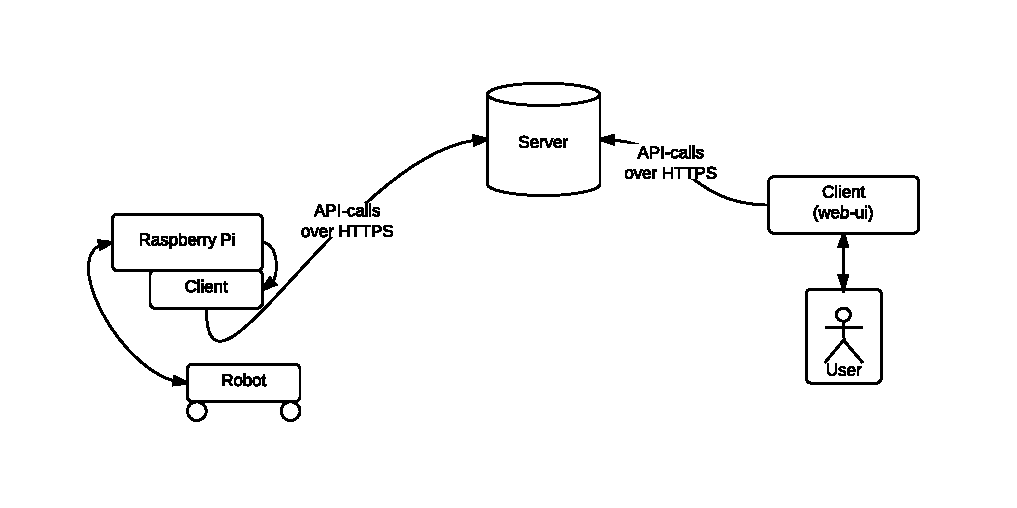
\includegraphics[width=\textwidth]{graphics/robot-implementation.pdf}
\caption{An overview of the demonstrated system and its hierarchy of components and how they interact.}
\label{fig:robot-implementation}
\end{figure}

The project was initially split into three parts:
``Server'',``agent (robot)'' and ``server-agent communication''.
The agent and server-agent communication are both part of the agent client, shown in Figure~\ref{fig:robot-implementation}.
At the concluding phase of the project, these three parts were connected and executed in unison to demonstrate the system.
The planning work done early proved to be very useful: the finishing phase was completed without issues.

A user client was implemented as a web-based graphical user interface usable from any modern web browser.
It can be accessed by both smartphones and computer, and from anywhere in the world. 
The robot's wheels and arm was successfully controlled via this interface.
Experienced latency was tolerable when controlling the vehicle while both the controller and agent was connected to NTNU's eduroam network, with the server on an off-site location.
However the system cannot guarantee real time performance on an arbitrary network, as no guarantees can be made about the worst case client-server latency as this is based on the clients' and server's internet connectivity.
The robot's error handling worked well: its behavior was as intended when we introduced various error conditions.

